% ------------------------------------------------------------------------------
% TYPO3 CMS 6.2 LTS - What's New - Chapter "Introduction" (Spanish Version)
%
% @author	Sergio Catalá <sergio.catala@e-net.info>
% @author	Michel Mix <mmix@autistici.org>
% @license	Creative Commons BY-NC-SA 3.0
% @link		http://typo3.org/download/release-notes/whats-new/
% @language	Spanish
% ------------------------------------------------------------------------------
% Standard Slide
% ------------------------------------------------------------------------------

\section{Introducción}
\begin{frame}[fragile]
	\frametitle{Introducción}

	\begin{center}\huge{Introducción}\end{center}
	\begin{center}\huge{\color{typo3darkgrey}\textbf{(Hechos Rápidos)}}\end{center}

\end{frame}

% ------------------------------------------------------------------------------
% TYPO3 CMS 6.2 LTS: The Facts (1)
% ------------------------------------------------------------------------------

\section{Introducción}
\begin{frame}[fragile]
	\frametitle{Introducción}
	\framesubtitle{TYPO3 CMS 6.2 LTS: Los Hechos (1)}

	\begin{itemize}
		\item Foco en:

			\begin{itemize}
				\item Migración Sin Problemas
				\item Base Robusta y Segura
				\item Bienestar del Usuario
				\item Tecnologías Modernas/Interoperabilidad
			\end{itemize}

	\end{itemize}

	\begin{columns}[T]

		\begin{column}{.5\textwidth}
			\begin{itemize}
				\item Gerente de Lanzamiento:
				\begin{itemize}
					\item Ernesto Baschny\newline
						ernesto.baschny (at) typo3.org\newline
						Twitter: @baschny
				\end{itemize}
			\end{itemize}
		\end{column}

		\begin{column}{.5\textwidth}
			\begin{figure}
				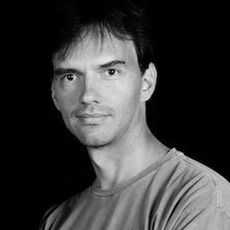
\includegraphics[width=2.6cm,height=2.6cm]{Images/Introduction/ErnestoBaschny.jpg}
			\end{figure}
		\end{column}

	\end{columns}

\end{frame}

% ------------------------------------------------------------------------------
% Standard Slide
% ------------------------------------------------------------------------------

\begin{frame}[fragile]
	% \TabPositions{1.2cm}

	\frametitle{Introducción}
	\framesubtitle{TYPO3 CMS 6.2 LTS: Los Hechos (2)}

	\begin{itemize}
		\item Fecha de lanzamiento: 25 Marzo 2014
		\item Desarrollo y línea de tiempo del lanzamiento:
	\end{itemize}

	\begin{figure}
		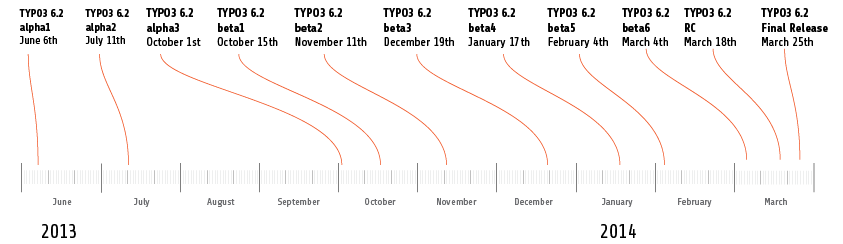
\includegraphics[width=0.99\linewidth]{Images/Introduction/ReleaseTimeline.png}
	\end{figure}

\end{frame}

% ------------------------------------------------------------------------------
% Standard Slide
% ------------------------------------------------------------------------------

\begin{frame}[fragile]
	\frametitle{Introducción}
	\framesubtitle{TYPO3 CMS 6.2 LTS: Los Hechos (3)}

	\begin{itemize}
		\item Requisitos del Sistema
		\begin{itemize}
			\item PHP	\tabto{1.2cm} v5.3.7 - v5.5.x
			\item MySQL	\tabto{1.2cm} v5.1.x - v5.6.x
		\end{itemize}
	\end{itemize}

	\begin{itemize}
		\item Fin de mantenimiento: Marzo 2017
		\item TYPO3 CMS 6.2 es un lanzamiento de \textbf{Soporte a Largo Plazo} (LTS) (¡3 años de soporte!)
	\end{itemize}

\end{frame}

% ------------------------------------------------------------------------------
% Standard Slide
% ------------------------------------------------------------------------------

\begin{frame}[fragile]
	\frametitle{Introducción}
	\framesubtitle{TYPO3 CMS 6.2 LTS: Los Hechos (4)}

	\begin{itemize}
		\item Agenda de lanzamiento TYPO3 CMS:
	\end{itemize}

	\begin{figure}
		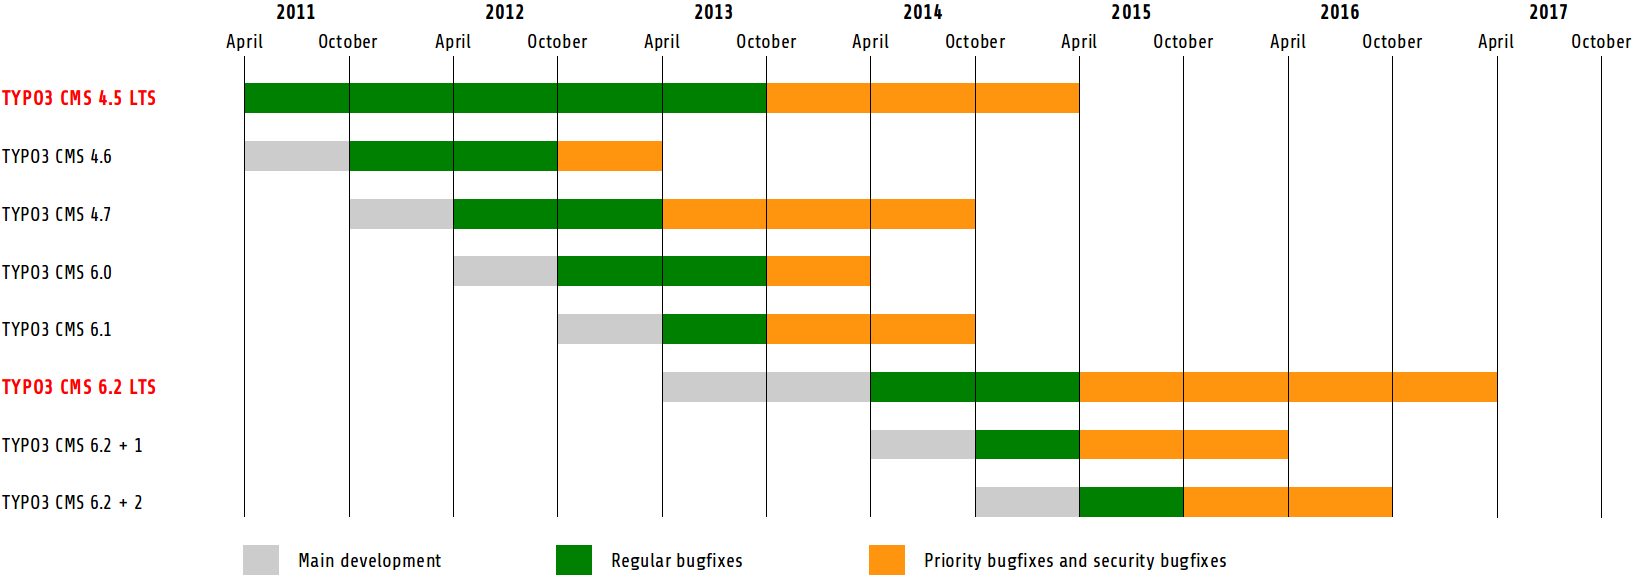
\includegraphics[width=0.99\linewidth]{Images/Introduction/ReleaseAgenda.png}
	\end{figure}

\end{frame}

% ------------------------------------------------------------------------------

